\documentclass{article}
\usepackage[utf8]{inputenc}
\usepackage[spanish.mexico]{babel}
\usepackage[american voltages, american currents,siunitx]{circuitikz}

%Plotting

\usepackage{pgfplots}

\pgfplotsset{width=10cm,compat=1.9} 
 \usepgfplotslibrary{external}
\tikzexternalize 

%Matematicas
\usepackage{amsmath}
\usepackage{mathtools}





\title{Formulario Comunicaciones Analógicas}
\author{Pablo Vivar Colina\\
Grupo 13
}
%\date{Septiembre 2017}

\usepackage{natbib}
\usepackage{graphicx}

\begin{document}

\maketitle

\section{Sinusoide}

En matemáticas se denomina sinusoide o senoide a la curva que representa gráficamente la función seno y también a dicha función en sí. Es una curva que describe una oscilación repetitiva y suave.\\

Su forma más básica en función del tiempo (t) es:\citep{Sinusoide}\\

\begin{equation}
    y(t) = A\sen(\omega t + \varphi)
\end{equation}

La senoide es importante en física debido al hecho descrito por el teorema de Fourier que dice que toda onda, cualquiera que se sea su forma, puede expresarse de manera única como superposición (suma) de ondas sinosuidales de longitudes de onda y amplitudes definidas. Por este motivo se usa esta función para representar tanto a las ondas sonoras como las de la corriente alterna.\citep{Sinusoide}\\

\subsection{Características}

La sinusoide puede ser descrita por las siguientes expresiones matemáticas:

\begin{equation}
y(x) = A\ {\rm{sen}}\left (\omega x + \varphi \right )
\end{equation}

\begin{equation}
y(t) = A\sen(2 \pi f t + \varphi)
\end{equation}


\begin{equation}
y(x) = A\ {\rm{sen}} \left (\frac {2\pi }{T}x + \varphi \right )
\end{equation}

donde:\\

\begin{itemize}
    \item $A$ es la amplitud de oscilación.
 \item $\omega$ es la velocidad angular  \item $\omega = 2\pi f$
  \item $f$ es la frecuencia de oscilación.
  \item $T$ es el período de oscilación  \item  $T = {1}/{f}$
 \item $\omega x$ + $\varphi$ es la fase de oscilación.
   \item $\varphi$ es la fase inicial.
\end{itemize}

\begin{figure}
    \centering
    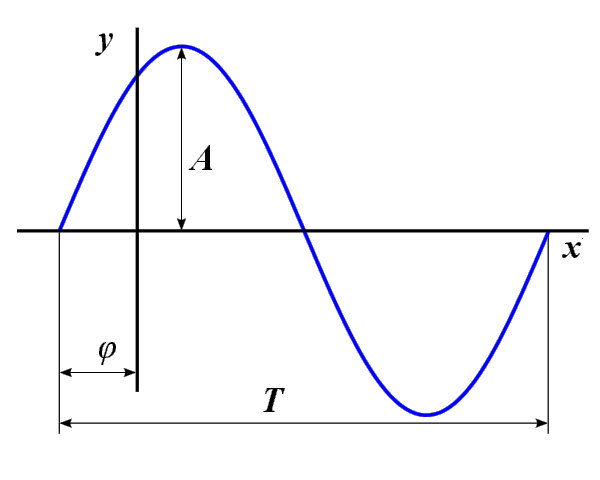
\includegraphics[width=0.6\textwidth]{Imagenes/Alg_sinusoide.png}
    \caption{Parámetros característicos de una forma sinusoidal.}
    \label{fig:parametro_sinusoide}
\end{figure}
 
 
 \section{Media Cuadrática}
 
 En matemáticas, la media cuadrática, valor cuadrático medio o RMS (del inglés root mean square) es una medida estadística de la magnitud de una cantidad variable. Puede calcularse para una serie de valores discretos o para una función matemática de variable continua. El nombre deriva del hecho de que es la raíz cuadrada de la media aritmética de los cuadrados de los valores.\citep{MediaCuadratica}\\

A veces la variable toma valores positivos y negativos, como ocurre, por ejemplo, en los errores de medida. En tal caso se puede estar interesado en obtener un promedio que no recoja los efectos del signo. Este problema se resuelve, mediante la denominada media cuadrática. Consiste en elevar al cuadrado todas las observaciones (así los signos negativos desaparecen), en obtener después su media aritmética y en extraer, finalmente, la raíz cuadrada de dicha media para volver a la unidad de medida original. La desviación estandar es una media cuadrática.\citep{MediaCuadratica}\\

\begin{equation}
    x_{\mathrm{rms}} = \sqrt {{1 \over {T_2 - T_1}} {\int_{T_1}^{T_2} {[f(t)]}^2\, dt}}. \qquad\qquad 
\end{equation}

%SEÑAL TRIANGULAR


\section{Señales}

\subsection{Señales determinísticas}

\subsubsection{Señal cuadrada}

La señal cuadrada se puede representar mediante la serie de fourier desarrollada:\citep{SeriesFourier}\\

\begin{equation}
    \oint_{\partial \Sigma} \mathbf{B} \cdot \mathrm{d}\boldsymbol{l} = \mu_0 \iint_{\Sigma} \mathbf{J} \cdot \mathrm{d}\mathbf{S} + \mu_0 \varepsilon_0 \frac{\mathrm{d}}{\mathrm{d}t} \iint_{\Sigma} \mathbf{E} \cdot \mathrm{d}\mathbf{S}
\end{equation}

\begin{equation}
    \frac{4}{\pi}[sin(\pi \omega_o t)+\frac{1}{3}sin(3 \pi \omega_o t)+\frac{1}{5}sin(5 \pi \omega_o t)+(\ldots)]
    \label{ecuacionCuadrada}
\end{equation}



como se vio en la ecuacion \ref{ecuacionCuadrada} se hizo lo siguiente

\begin{figure}[h!]
    \centering

\begin{tikzpicture}
\begin{axis}[
    axis lines = left,
    xlabel = {t[s]},
    ylabel = {V[V]},
]


\addplot
[thick=0.1cm,
    domain=0:0.1, 
    samples=100, 
    color=green,
]
{(4/3.14159265359)*(sin(2*3.14159265359*1000*x)+(1/3)*sin(3*2*3.14159265359*1000*x)+(1/5)*sin(5*2*3.14159265359*1000*x)};
%+(1/7)*sin(7*2*3.14159265359*1000*x)+(1/9)*sin(9*2*3.14159265359*1000*x)+(1/11)*sin(11*2*3.14159265359*1000*x)+(1/13)*sin(13*2*3.14159265359*1000*x)+(1/15)*sin(15*2*3.14159265359*1000*x))

%Se añade nota :D
%\addlegendentry{[1]}

\end{axis}
\end{tikzpicture}
\caption{Señal cuadrada unitaria}
\label{Senalcuadrada20pp}
\end{figure}
%%

\subsubsection{Señal onda triangular}

La señal cuadrada se puede representar mediante $\Omega$ la serie de Fourier desarrollada:\citep{SeriesFourier}\\

\begin{equation}
    \frac{\pi}{2} - \frac{4}{\pi}[\frac{cos(\omega_o t)}{1^2}+\frac{cos(3\omega_o t)}{3^2}+\frac{cos(5\omega_o t)}{5^2}+(\ldots)]
\end{equation}

\begin{figure}[h!]
    \centering

\begin{tikzpicture}
\begin{axis}[
    axis lines = left,
    xlabel = {t[s]},
    ylabel = {V[V]},
]


\addplot
[thick=0.1cm,
    domain=0:0.1, 
    samples=100, 
    color=blue,
]
{ (3.14159265359/2)-(4/3.14159265359)*(((cos(2*3.14159265359*1000*x))/1)+((cos(3*2*3.14159265359*1000*x))/9))
};
%+((cos(5*2*3.14159265359*1000*x))/25)+((cos(7*2*3.14159265359*1000*x))/49)+((cos(9*2*3.14159265359*1000*x))/81)+((cos(11*2*3.14159265359*1000*x))/121)

%Se añade nota :D
%\addlegendentry{[1]}

\end{axis}
\end{tikzpicture}
\caption{Señal cuadrada unitaria}
\label{SenalTriangular20pp}
\end{figure}
%%



\section{Distribucion noraml}




\subsubsection{Armónicas}

\subsubsection{Intermodulación}

\subsection{Distorsión Alineal}

\subsubsection{Ganancia}

\subsubsection{Fase}



\bibliographystyle{plain}
\bibliography{Referencias.bib}


\end{document}